%%=============================================================================
%% Methodologie
%%=============================================================================

\chapter{\IfLanguageName{dutch}{Methodologie}{Methodology}}%
\label{ch:methodologie}


\lstset{
    language=yaml
    basicstyle=\ttfamily,
    columns=fullflexible,
    frame=single,
    breaklines=true
}
%% TODO: Hoe ben je te werk gegaan? Verdeel je onderzoek in grote fasen, en
%% licht in elke fase toe welke stappen je gevolgd hebt. Verantwoord waarom je
%% op deze manier te werk gegaan bent. Je moet kunnen aantonen dat je de best
%% mogelijke manier toegepast hebt om een antwoord te vinden op de
%% onderzoeksvraag.



Na de eerste studie van alle betrokken onderdelen, zijnde Big Data, Docker (Compose), Kubernetes, VIC infrastructuur, zien we 2 mogelijke manieren om dit alles op te zetten en dienen we te beslissen op welke manier we het gaan aanpakken. In dit eerste deel gaan we dieper in op die keuze.

\section{Welke omgeving gaan we opzetten?}

Bij elk platform is het de bedoeling de gebruikers een aangename ervaring te bieden, daarbij is performantie een belangrijk onderdeel, vooral bij Big Data oplossingen waar het verwerken van grote volumes data veel tijd kost en soms in bijna real-time dient te gebeuren.
In het streven naar goede performantie speelt Schaalbaarheid een belangrijke rol, en de architectuur van Hadoop, Spark en Kafka ondersteunt volop het inschakelen van extra 'machines' bij een toenemend aantal gebruikers en behoefte aan meer snelheid en verwerkingscapaciteit.
Bij een typische installatie van deze oplossingen zou een cluster van elk opgezet worden. Elke cluster kan onafhankelijk op- en neerschalen naargelang de nood.
\newline
\newline
De schaalbaarheid bij Spark bijvoorbeeld, is doordat het werk verdeeld wordt over meerdere Executors en er dus in een cluster eenvoudig extra Executors kunnen gebruikt worden. Zie ook volgende figuur.
\newline
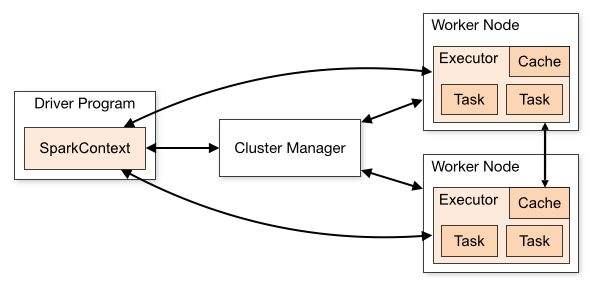
\includegraphics[scale=0.7]{cluster-overview.png}
\newline
Een van de onderdelen van Hadoop is YARN, een resource manager en job scheduler die instaat voor de verdeling van het werk over de verschillende cluster nodes en dus zorgt voor de schaalbaarheid.
\newline
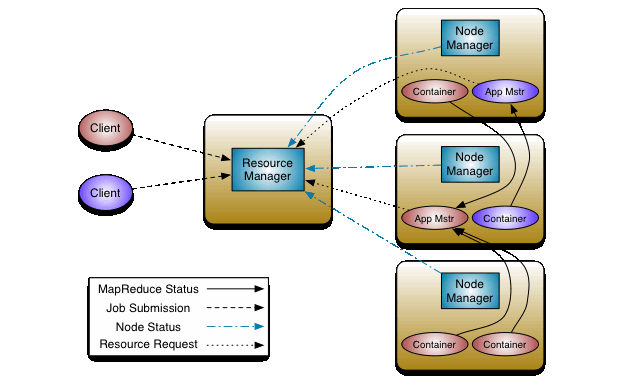
\includegraphics[scale=0.7]{yarn_architecture.png}
\newline
Bij elk van de gebruikte applicaties moeten dus een aanzienlijk aantal nodes opgezet worden: gedefinieerd, geconfigureerd en geïnstalleerd. Kubernetes is een platform dat typisch hiervoor wordt gebruikt. Spark bijvoorbeeld kan rechtstreeks gebruikmaken van Kubernetes. Daarbij werkt Spark rechtstreeks met Kubernetes om Executors op Kubernetes Pods aan te maken en er applicaties op uit te voeren.
\newline
https://spark.apache.org/docs/latest/running-on-kubernetes.html
\newline
\newline
Merk op dat het bij een real-world installatie van combinaties van deze 3 clusters, het meestal de bedoeling is dat de Big Data oplossingen achterliggend gebruikt wordt door eigen applicaties en dat gewone gebruikers op geen enkele manier rechtstreeks toegang krijgen to bv. Hadoop of Spark. Bij de meeste installaties volstaat dan ook het om als beveiliging de netwerk toegang tot de Big Data oplossingen te beperken.
\newline
\newline
Eén van de doelstellingen van deze bachelorproef is om de verschillende gebruikers (studenten), zowel tijdens de les als tijdens examens volledig afgezonderd te laten werken. Die afzondering geldt zowel op gebied van security als stabiliteit.

\subsection{Security}

\subsubsection{Hadoop Secure mode} (https://hadoop.apache.org/docs/stable/hadoop-project-dist/hadoop-common/SecureMode.html)
In een standaard configuratie wordt de Hadoop cluster beschermd door alle netwerk toegang te beperken. Als er daarnaast ook nog restricties nodig zijn op wie toegang krijgt tot de cluster om gegevens te bekijken of applicaties te beheren, moeten authenticatie en toegang tot de cluster volledig geconfigureerd worden. Bij een Hadoop cluster die in 'secure mode' is opgezet, dient er voor elke Hadoop service en elke gebruiker authenticatie te gebeuren door Kerberos, een extra oplossing die dit ondersteund is dan nodig.
\newline
\newline
'Forward and reverse host lookup for all service hosts must be configured correctly to allow services to authenticate with each other. Host lookups may be configured using either DNS or /etc/hosts files.'
\newline
\newline
Volgens de documentatie is een goede kennis van Kerberos en DNS vereist om Hadoop services op te zetten in 'secure mode'.
\newline
\newline
\subsubsection {Spark authenticatie en authorisatie} (https://spark.apache.org/docs/latest/security.html) \newline
Net zoals bij Hadoop zijn Security functionaliteiten zoals authenticatie niet actief bij een standaard installatie van Spark. Als er beperking is van de geen netwerk toegang, moet communicatie tussen de Spark processen afgeschermd worden d.m.v. authenticatie en encryptie, lokale opslag moet ook encryptie gebruiken. De Web User Interface moet beschermd worden door Authenticatie, en daarvoor moeten Java servlet filters gebruikt worden, die echter niet door Spark worden aangeboden en dus moeten gebouwd worden op maat van het systeem dat de authenticatie zal doen.
Er zijn voorbeelden te vinden van dit soort filters, meestal gebaseerd op Basic Authentication (zie verder bij nginx). Volgende blog heeft ook een filter gebouwd die een login pagina gebruikt: \newline https://blog.cacoveanu.com/2019/2019.02.11.spark\_ui\_authentication.html
\newline
\newline
Gebruikers afschermen van elkaar in een opstelling van Hadoop, Spark, Kafka, allemaal in clusters wordt snel zeer ingewikkeld. Elk van de oplossingen bestaat uit meerdere processen die met elkaar communiceren en ieder onderdeel moet secure opgezet worden zodat gebruikers niet, bewust of per ongeluk, data van elkaar te zien krijgen. We spreken hier over encryptie voor de opslag, authenticatie en encryptie bij communicatie tussen de verschillende processen, authenticatie voor de gebruiker op Hadoop, authenticatie voor de gebruiker op Spark enz.
De manier van beveiligen is voor elk van deze oplossingen en interne processen op een andere manier, en vraagt om bijkomende softwares zoals LDAP, Kerberos server, enz.

\subsection{Stabiliteit}

Elk van de Big Data oplossingen, en Kubernetes, ondersteunen mechanismes om applicaties te verdelen over de pods en van elkaar af te schermen, bij bepaalde onderdelen kunnen er limieten gezet worden op CPU en geheugen gebruik. Deze configuraties zijn gekoppeld aan nodes, containers en applicaties. De achterliggende bedoeling is vooral om eigen gebouwde applicaties te ondersteunen en vlot te laten beroep doen op de Big Data functionaliteiten. De focus ligt minder op rechtstreeks gebruik van de oplossingen door gebruikers die applicaties aan het ontwikkelen zijn.

Aangezien het de bedoeling is om de oefeningen van de studenten zoveel mogelijk van elkaar gescheiden te houden, o.a. om te vermijden dat slechte code van 1 student de applicaties crasht of overbelast, gaan we op basis van de docker-compose files voor elke student een aparte omgeving creëren. Dit betekent dat elke applicatie/container voor elke student apart wordt opgestart maar het is niet de bedoeling dat dit manueel gebeurt, hiervoor bestaat software die toelaat om het beheer van containers te doen, op een automatische manier op te starten, monitoren, herstarten, afsluiten, enz.



\subsection{Conclusie}

Een gedeelde cluster leek mij noch voor de Security, noch voor de Stabiliteit vereisten de beste aanpak voor de cursus Big Data, gezien het vele werk en de complexiteit om dit alles juist te configureren, en het risico dat niet alle resources 100\% afgeschermd zijn van onbetrouwbare applicaties. Binnen de beperkte tijd voor de uitwerking van de bachelorproef is dit niet mogelijk.
\newline
\newline
Daarbij komt dat het gebruik van de Big Data oplossingen hier niet in het kader is van een eigen afgewerkte applicatie die aan eindgebruikers wordt aangeboden, maar dat ze eerder als een Development omgeving aangeboden wordt aan de studenten. En voor een Development omgeving wordt, dankzij de flexibiliteit van containertechnologie, dikwijls gekozen voor een persoonlijke omgeving per ontwikkelaar. Deze omgeving kan dan lokaal of in de cloud zijn.
\newline
\newline
De mogelijkheden die een cluster biedt, de schaalbaarheid en alle resources optimaal gebruiken, om applicaties zo efficient mogelijk te ondersteunen zijn tijdens Development minder van belang. Belangrijker is de onafhankelijkheid en flexibiliteit van de eigen omgeving.
Dus ik denk dat het hier ook beter, en eenvoudiger, is om elke student een eigen omgeving te geven, volledig afgeschermd van de andere, door aparte containers te gebruiken per student.
\newline
\newline
De nodige combinaties van containers, nodig voor de oefeningen of examen, kunnen we opzetten door gebruik te maken van Docker Compose files die een specifieke combinatie definiëren van de Big Data oplossingen. Voor elke student wordt dan een omgeving apart opgestart, door gebruik te maken van vSphere Virtual Containers, vSphere Pods of Kubernetes. Merk op dat de Docker Compose file het startpunt is voor elk van deze omgevingen, maar dat een pure Docker Compose niet voldoende is. De basis dient uitgebreid te worden met specifieke configuraties gerelateerd aan de omgeving, zoals definitie van netwerken en adressen, volumes, enz.
\newline
\newline
Een bijkomend voordeel van deze aanpak, elke student een eigen setup, is dat een omgeving niet alleen kan gebruikt worden om applicaties op de Big Data oplossingen te ontwikkelen, maar ook om studenten de administratie van de Big Data oplossingen zelf op hun eigen geïsoleerde omgeving te leren. Op hun eigen omgeving kunnen ze Admin zijn zonder impact op anderen.

\section{VIC}

De infrastructuur van VIC HoGent is gebaseerd op VMware vSphere (VMware's virtualization platform), waarvan de 2 belangrijkste onderdelen ESXi en vCenter Server zijn. ESXi is het virtualisatie platform waar virtuele machines worden uitgevoerd en vCenter Server is de service waarmee alles beheerd wordt.
\newline
\newline
De vSphere oplossing is leider in traditionele virtualisatie, gebaseerd op Virtuele machines. Applicatie virtualisatie, waarbij elke applicatie in een aparte container draait, wordt steeds belangrijker (zie hoofdstuk 2), en voor dit soort aanpak zijn Docker containers de standaard oplossing.
\newline
\newline
Om hieraan tegemoet te komen werd door VMWare voor vSphere 6 'vSphere Integrated Containers' ontwikkeld, een oplossing die toelaat om Docker images en containers te gebruiken op bestaande vSphere infrastructuur. Toevallig noemt dit ook VIC.
Deze oplossing ondersteunt ook het deployen van Multi-Container Applicaties, o.a. door het gebruik van Docker Compose files. (https://vmware.github.io/vic-product/assets/files/html/1.3/vic\_app\_dev/deploy\_multiple\_docker\_compose.html)
\newline
\newline
Intussen is Kubernetes de de-facto standaard geworden voor de orchestratie en het beheer van containers op grote schaal.
\newline
\newline
Dus zijn Docker containers en Kubernetes nu geïntegreerd vanaf vSphere versie 7. Dit op 2 manieren, ofwel door gebruik van vSphere Pods waarbij het beheer nog steeds via de traditionele vSphere Admin verloopt, ofwel door Tanzu Kubernetes cluster. Dit is software van VMWare die apart wordt geïnstalleerd en die de Kubernetes manier van werken ondersteunt en dus ook meer controle biedt over het beheer van de Kubernetes cluster.
De 'vSphere Integrated Containers' oplossing van vSphere 6 wordt niet langer ondersteund en ook Docker Compose niet meer.
\newline
\newline
Zelf werken op de infrastructuur van VIC HoGent kan enkel onder supervisie en binnen beperkte tijden. Gezien mijn stage in combinatie met mijn bachelorproef was dit moeilijk en daarnaast was de beschikbaarheid van mijn co-promoter ook beperkt dus is er afgesproken dat ik de nodige informatie zou bezorgen die aantoont dat Kubernetes kan gebruikt worden op vSphere en zelf al het werk op een lokale Kubernetes installatie zou uitvoeren.

\section{Big data}

Om meer vertrouwd te geraken met de Big Data oplossingen heb ik ze eerst allemaal eens lokaal opgezet via Docker Compose configuraties. Zie Appendix [TODO].
Daarbij ben ik vertrokken van voorbeelden die beschikbaar zijn op het Internet en voorbeelden uit de Big Data cursus oefeningen.
\newline
\newline
Dit verliep vlot. Pas wanneer ik ze begon om te zetten naar Kubernetes, zie verder, heb ik gemerkt dat het gebruik van Docker en Docker Compose lokaal voor heel wat voordelen zorgt. Bijvoorbeeld dat je eenvoudig een shell kunt openen in om het even welke lokale Docker container en daar commandos kunt uitvoeren die gebruik maken van de geïnstalleerde software in die container. Dit wordt voor de oefeningen gebruikt om bijvoorbeeld Hadoop commandos uit te voeren terwijl er op de lokale machine geen hadoop beschikbaar is. Via 'docker exec' kan de student op de lokale Namenode container aanloggen, er files naar kopiëren en die dan via 'hadoop' commandos naar hdfs in de andere container overbrengen, of Java programma's opstarten.

\section{Security}

We gaan dus niet voor een volledige, alle producten, alle processen, alle communicatie, secure installatie want 1 enkele omgeving voor 1 student zal volledig binnen 1 pod draaien en dus in eerste instantie ook volledig afgeschermd zijn.
De uitdaging is nu eerder om bepaalde poorten toegankelijk te maken om toe te laten met deze omgeving te werken, maar we willen de toegang tot deze poorten voor elke omgeving wel beperken tot 1 student.

\subsection{Apache Knox}

Een oplossing die toe laat een Hadoop cluster af te schermen is Apache Knox\newline (https://knox.apache.org/). Dit is een gateway die de toegang tot de cluster vormt voor alle interacties (REST en HTTP), en die authenticatie doet van de gebruikers. Voor die authenticatie worden de typische protocols ondersteunt zoals LDAP/ActiveDirectory, Kerberos, SAML en OAuth. Dit is ideaal in een onderneming om bestaande gebruikers toe te laten, maar voelt overdreven (overkill) in ons geval van 1 gebruiker per omgeving. Ik zocht dus naar iets eenvoudigere.

\subsection{Nginx}

Nginx (https://www.nginx.com/) is een web server die dikwijls als ingangspunt van een web site gebruikt wordt (Reverse proxy - https://en.wikipedia.org/wiki/Reverse\_proxy) en die zorgt dat de achterliggende structuur afgeschermd is voor de buitenwereld. Daarnaast kan het zorgen voor Load Balancing (https://nl.wikipedia.org/wiki/Load\_balancing) en beveiliging (HTTP Basic Authentication, SSL/TLS offloading).
\newline
\newline
HTTP Basic Authentication (https://en.wikipedia.org/wiki/Basic\_access\_authentication)
Basic Authentication is een optioneel onderdeel van een HTTP(S) transactie waarbij aan de initiërende partij, typisch de webbrowser, gevraagd wordt een gebruikersnaam en paswoord te verstrekken. Het is de eenvoudigste techniek voor het afdwingen van toegangscontroles tot web resources, omdat hiervoor geen cookies, sessie-ID's of inlogpagina's nodig zijn.
Omdat de inloggegevens in de header van elk HTTP(S)-verzoek moeten worden verzonden, moet de webbrowser ze gedurende een redelijke tijd in de cache opslaan om te voorkomen dat de gebruiker voortdurend om zijn gebruikersnaam en wachtwoord wordt gevraagd.
Merk op dat de inloggegevens die verstuurd worden (gebruikersnaam en paswoord) niet beschermd zijn, ze zijn gecodeerd met base64 encoding maar dit biedt geen enkele bescherming. Daarom wordt Basic Authentication meestal gebruikt in combinatie met HTTPS om vertrouwelijkheid te bieden. Aangezien het in onze oplossing over tijdelijke omgevingen gaat is het gevaar dat bij HTTP de inloggegevens onderschept worden minimaal en kan dit dus ook voor niet-HTTPS gebruikt worden.
\newline
\newline
Basic Authentication lijkt me voldoende, per omgeving moeten dan de inloggegevens voor 1 gebruiker, de student, opgezet worden. Nginx ondersteunt meerdere mechanismen voor authenticatie waaronder een eenvoudige paswoord file. Deze is in het formaat
\newline
\newline

\begin{lstlisting}
user1:$apr1$/woC1jnP$KAh0SsVn5qeSMjTtn0E9Q0
user2:$apr1$QdR8fNLT$vbCEEzDj7LyqCMyNpSoBh/
user3:$apr1$Mr5A0e.U$0j39Hp5FfxRkneklXaMrr/ 

\end{lstlisting}

en wordt gegenereerd door Linux tools zoals htpasswd (deel van apache2-utils en httpd-tools), waarbij het paswoord van een gebruiker met MD5 wordt geëncrypteerd. In ons geval zou deze file dus de unieke student gebruiker bevatten, met verschillend paswoord per omgeving.
Optioneel kan overal een extra account voor de lesgever, met identiek paswoord voor alle omgevingen, toegevoegd worden.
\newline
\newline
Als eerste onderzoek voor dit security onderdeel heb ik, om de configuratie van de Basic Authenticatie te bouwen, een beperkte Kubernetes yaml file gemaakt met alleen maar nginx, deze start en stopt snel tijdens het testen, maar liet al direct toe om Kubernetes Services, Port mapping en Configmap te gebruiken. Dit was ook de eerste keer dat ik Kubernetes ben beginnen te gebruiken en die dus lokaal heb geïnstalleerd.
\newline
\newline
Configmaps (https://kubernetes.io/docs/concepts/configuration/configmap/)
Een ConfigMap wordt gebruikt om niet-beveiligde configuratie gegevens te beheren en ter beschikking te stellen van Containers, als environment variabele of als (configuratie) file via een volume.
\newline
\newline
Initieel had ik hier problemen met het configureren van de volumes omdat Kubernetes volumes op een andere manier werken dan de volumes van Docker Compose, waar er eenvoudig verwezen kan worden naar lokale folders op de machine waar de container draait, terwijl bij Kubernetes alles in de Configmap gestopt wordt om op die manier van Pod te kunnen switchen of uitbreiden, en de configuratie (files) mee moet kunnen naar alle pods.
\newline
\newline
In de ConfigMap heb ik de nginx.conf file gestopt en de paswoord file voor Basic Authentication.
Uiteindelijk met volgende configuratie kreeg ik de popup voor Basic Authentication.
\newpage
\begin{lstlisting}
user  nginx;
worker_processes  1;

error_log  /var/log/nginx/error.log warn;
pid        /var/run/nginx.pid;

events {
    worker_connections  1024;
}
http {
    include       /etc/nginx/mime.types;
    
    default_type  application/octet-stream;
    
    log_format  main  '$remote_addr - $remote_user [$time_local] "$request" '
    '$status $body_bytes_sent "$http_referer" '
    '"$http_user_agent" "$http_x_forwarded_for"';
    
    access_log  /var/log/nginx/access.log  main;
    
    sendfile        on;
    
    keepalive_timeout  65;
    
    server {
        listen 443 ssl;
        listen [::]:443 ssl;
        
        server_name         www.hadoop.local;
        ssl_certificate     /etc/nginx/ssl/tls.crt;
        ssl_certificate_key /etc/nginx/ssl/tls.key;
        ssl_protocols       TLSv1 TLSv1.1 TLSv1.2;
        ssl_ciphers         HIGH:!aNULL:!MD5;
        
        proxy_set_header Host $host;
        proxy_set_header X-Forwarded-For $proxy_add_x_forwarded_for;
        
        proxy_cache_revalidate on;
        proxy_cache_use_stale error timeout http_500 http_502 http_503 http_504;
        proxy_cache_background_update on;
        proxy_cache_lock on;
        
        resolver kube-dns.kube-system.svc.cluster.local valid=5s;
        
        auth_basic "Access restricted";
        auth_basic_user_file /etc/nginx/password.conf;
        
        location / {
            root /usr/share/nginx/html;
            index index.html index.htm;
        }
    }
}
\end{lstlisting}

[TODO] - Eigen image voor nginx docker + config via ENV
https://github.com/dtan4/nginx-basic-auth-proxy
\newline
\newline
\begin{lstlisting}
version: '2'
services:
web:
image: tutum/hello-world:latest
nginx:
image: quay.io/dtan4/nginx-basic-auth-proxy:latest
ports:
- 8080:80
- 8090:8090
environment:
- BASIC_AUTH_USERNAME=username
- BASIC_AUTH_PASSWORD=password
- PROXY_PASS=http://web/
- PROXY-SERVERNAME=hadoop.student1.hogent.be
\end{lstlisting}

\section{Hadoop}

Daarna heb ik Hadoop toegevoegd en de configuratie voor nginx om als Reverse Proxy gebruikt te worden voor Hadoop. Hierbij was ik vertrokken van de Docker Compose file die ik had opgebouwd en getest in vorige stappen, en heb die toegevoegd aan de Kubernetes file maar bij het opstarten waren er een aantal problemen. De namenode was niet bereikbaar voor de datanode, resourcemanager en historyserver.
In een Docker compose file worden alle containers verbonden via 1 of meerdere virtuele netwerken, en zorgt Docker ervoor dat de containers naar elkaar kunnen verwijzen door middel van de containernaam. Dit is niet het geval bij Kubernetes (of vSphere), waar de naam van de Pod, waarop de container draait, moet worden gebruikt. Aangezien in onze oplossing alle containers voor 1 student op dezelfde Pod draaien kunnen we ook 'localhost' gebruiken.\newline
In de configuratie voor Kubernetes moest ik dus bij elke container de verwijzing naar andere containers (hostnamen) vervangen door 'localhost'.
\newline
\newline
Om de configuratie van Hadoop aan te passen zijn er 2 manieren, ofwel gebruikmakende van environment variabelen gedefinieerd rechtstreeks op de container ofwel met environment variabelen gedefinieerd in een aparte ConfigMap. Typisch worden beiden gebruikt, in de ConfigMap stoppen we variabelen die voor alles containers gelijk zijn, op de container de variabelen die verschillend zijn per container. Een voorbeeld van de laatste soort is SERVICE\_PRECONDITION die een manier is om de bepalen op welke andere containers moet gewacht worden. Dit is een mechanisme van Apache, waarbij een specifieke applicatie wacht met opstarten tot het contact krijgt met die andere applicatie.
\newline
\newline
Na deze aanpassingen leek het nog niet voldoende om alles werkend te krijgen maar uiteindelijk bleek het te liggen aan de ConfigMap die ook nog elementen van nginx bevatte.
\newline
\newline
Eens Hadoop werkende in Kubernetes, begon ik met de reverse proxy configuratie van nginx. Eerst heb ik geprobeerd om een Hadoop context toe te voegen aan de URL, bv http://localhost/hadoop, en die via de nginx proxy\_pass door te sturen naar Hadoop.
\newline
\newline
\begin{lstlisting}
location / {
    proxy_set_header Host $http_host;
    proxy_redirect off;
    # rewrite ^/hadoop/(.*)$ /$1 break;
    proxy_pass http://localhost:9870/;
}

\end{lstlisting}

Daarbij kreeg ik volgende probleem:
\newline
\newline
- Browser vraagt http://localhost/hadoop
- Browser krijgt HTML terug van Hadoop, via nginx
- HTML bevat verwijzingen naar /static/bootstrap.css
\newline
\newline
Een mogelijke oplossing hiervoor is ofwel nginx de HTML te laten aanpassen (filteren) en regels te definiëren die overal '/hadoop' toevoegen aan links van images, css, enz. Hierbij is er een kans dat we niet alle gevallen vinden en toevoegen aan de filter.
Een andere oplossing is om een apart DNS adres (servernaam) te gebruiken voor Hadoop, nginx kan dan op basis van de servernaam de requests doorsturen naar Hadoop. Hiervoor moest ik lokaal de hosts file van Windows (C:/Windows/System32/drivers/etc) wijzigen en het volgende toevoegen:
127.0.0.1 www.hadoop.local
\newline
\newline
De reverse proxy configuratie moest ook aangepast worden omdat het niet langer op url (location /hadoop) werkt maar op servernaam.
\newline
\newline
\begin{lstlisting}
server {
    listen 80;
    listen [::]:80;
    server_name localhost;
}
\end{lstlisting}

Toen ik daarna in de browser naar http://www.hadoop.local ging, kreeg ik eerst de user/paswoord popup en na invullen van de correcte gegevens zag ik de WebUI van Hadoop.

\section{HTTPS/SSL}

Om de installatie veiliger te maken is er beslist om HTTPS op te zetten. Het is voldoende om dit op nginx te configureren want dat is de enige server en communicatie die van buitenaf zichtbaar is en dus mogelijk kan bespioneerd worden. Er zijn nog een aantal voordelen dat dit enkel op de nginx server moet gebeuren:
\newline
\newline
- Performantie: SSL maakt zwaar gebruik van de CPU en op deze manier worden de andere containers hiermee niet belast.
- Certificaat beheer: installatie en onderhoud van de certificaten moet maar op 1 plaats gebeuren
- SSL software patching: indien kwetsbaarheden ontdekt worden in de SSL software moet de installatie van security patches enkel op de nginx gebeuren, eenvoudig door naar een nieuw image te verwijzen.
\newline
\newline
Het opzetten van SLL op een aparte server, nginx in dit geval noemt men 'SSL offloading'.

\subsection{Certificaat}

Om SSL op te zetten bij nginx is een certificaat nodig. Voor mijn lokale testen heb ik er zelf een gegenereerd gebruikt makende van openssl. Aangezien dit niet standaard al op Windows geïnstalleerd is, heb ik tijdelijk een Docker image gebruikt: alpine/openssl.
\newline
\newline
Met volgende commando kon ik een certificaat aanmaken dat vanuit de Docker container bewaard werd op mijn laptop.
\newline
\newline

docker run -ti --rm -v \$(pwd):/apps -w /apps alpine/openssl <openssl\_command>

\begin{lstlisting}
server {
    listen              443 ssl;
    server_name         www.hadoop.local;
    ssl_certificate     /etc/nginx/ssl/tls.crt;
    ssl_certificate_key /etc/nginx/ssl/tls.key;
    
    location / {
        proxy_pass ...
    }
}
\end{lstlisting}

\section{Spark}

Ik ben daarna begonnen met een Kubernetes yaml file te maken voor de combinatie Nginx, Hadoop en Spark. Dit verliep vlot, dezelfde problemen als bij Hadoop, vooral docker container namen die omgezet moesten worden naar localhost, enz die we intussen al snel herkenden.
\newline
\newline
Docker Compose biedt een functionaliteit die in Kubernetes niet bestaat, namelijk 'depends\_on'. Deze laat toe om de afhankelijkheid van containers te definiëren zodat containers niet starten voordat andere nodige containers zijn gestart. Dit wordt gebruikt bij Spark worker die (depends\_on) Spark master nodig heeft.
Bij Hadoop wordt dit opgelost door een eigen aanpak, de SERVICE\_PRECONDITION (zie eerder vermeld bij Hadoop).
\newline
\newline
Spark heeft daar geen oplossing voor maar uiteindelijk bleek dat de Spark processen hier geen hinder van ondervonden en dus het gebrek aan de 'depends\_on' geen probleem vormt.
\newline
\newline
Net zoals bij Hadoop heb ik dan bij nginx een servernaam geconfigureerd voor de reverse proxy, en de naam lokaal toegevoegd aan de hosts file:
127.0.0.1 www.spark.local
\newline
\newline
Toen ik daarna in de browser naar https://www.spark.local ging, kreeg ik eerst de user/paswoord popup en na invullen van de correcte gegevens zag ik de WebUI van Spark.

\section{Kafka}

Als laatste heb ik Kafka en Zookeeper opgezet in een Kubernetes configuratie. Ook hier weer zat de complexiteit in het vervangen van de juiste servernaam configuraties door localhost en openzetten van de juiste poorten.
Dit is nog een verschil met Docker Compose, namelijk de containers in een Compose file kunnen vrij met elkaar communiceren over alle poorten, de poorten die in een Compose gedefinieerd worden zijn de poorten die van buitenaf toegankelijk moeten zijn, bij Kubernetes moeten alle nodige poorten ook op elke container opengezet worden via configuratie.
\newline
\newline
Ik was als voorbeeld vertrokken van een configuratie met 3 Kafka brokers maar dit werd te zwaar voor mijn laptop in combinatie met alles van Kubernetes. Bij wijzigen van configuratie en herstarten van containers ging de Disk usage regelmatig naar 100% en moest ik mijn laptop herstarten.
Dus heb ik daarna een opzet gedaan met 1 Kafka broker en 1 Zookeeper.
\newline
\newline
Kafka ondersteunt meerder beveiligingsmechanismes waaronder SASL/PLAIN, een eenvoudige authenticatie gebaseerd op gebruikersnamen en paswoorden in een file.
\newline
\newline
Dit kan opgezet worden in een ConfigMap, dit is niet meer gebeurd door tijdsgebrek. (Voorlopig)
\newline
\newline
[TODO]
\begin{lstlisting}
KafkaReadExample.java
Dataset<Row> messages = spark.readStream()
.format("kafka")
.option("kafka.bootstrap.servers", BOOTSTRAP_SERVERS)
.option("subscribe", topic)
.option("", )
.option("", )
.option("", )

"kafka.sasl.jaas.config": 'org.apache.kafka.common.security.plain.PlainLoginModule required username="USERNAME" password="PASSWORD";',
"kafka.sasl.mechanism": "PLAIN",
"kafka.security.protocol" : "SASL_SSL",
\end{lstlisting}
\begin{lstlisting}
ConsumerDemo.java
properties.setProperty(, );
\end{lstlisting}
\section{Toestand}

- Volledig afgeschermd
- Enkel WEB UI beveiligd toegankelijk

\subsection{Testen}
\section{Mogelijke TODO}
hadoop commandos

\subsection{SSH/Hadoop container}

Indien nodig om hadoop commandos uit te voeren zonder lokaal te installeren.



\subsection{Kafka security}

\subsection{ssh container met hadoop}
\begin{lstlisting}
"kafka.sasl.jaas.config": 'org.apache.kafka.common.security.plain.PlainLoginModule required username="USERNAME" password="PASSWORD";',
"kafka.sasl.mechanism": "PLAIN",
"kafka.security.protocol" : "SASL_SSL",
\end{lstlisting}
\subsection{Spark lees/schrijven op hdfs}
 (org.apache.spark.sql)
In the mapping task, set the Spark session property spark.driver.extraJavaOptions to the following value: -Dhttp.proxyHost=<host> -Dhttp.proxyPort=<port> -Dhttp.proxyUser=<user> -Dhttp.proxyPassword=<password>

\subsection{Spark submit van applicatie op Hadoop Yarn}

\subsection{Documentatie voor installatie}

- Scripts/Optimalisatie voor installatie
- Voor meerdere studenten
- Op vSphere

\subsection{Conclusie}

- Op Kubernetes
- Lokaal install + yaml files
- Veel aandacht voor detail, configmap, etc
- Localhost / communicatie

Lokale Kubernetes